
\let\negmedspace\undefined
\let\negthickspace\undefined
\documentclass[journal,12pt,twocolumn]{IEEEtran}
\usepackage{cite}
\usepackage{amsmath,amssymb,amsfonts,amsthm}
\usepackage{algorithmic}
\usepackage{graphicx}
\usepackage{textcomp}
\usepackage{xcolor}
\usepackage{txfonts}
\usepackage{listings}
\usepackage{enumitem}
\usepackage{mathtools}
\usepackage{gensymb}
\usepackage[breaklinks=true]{hyperref}
\usepackage{tkz-euclide} % loads  TikZ and tkz-base
\usepackage{listings}
\usepackage{float}

\DeclareMathOperator*{\Res}{Res}
%\renewcommand{\baselinestretch}{2}
\renewcommand\thesection{\arabic{section}}
\renewcommand\thesubsection{\thesection.\arabic{subsection}}
\renewcommand\thesubsubsection{\thesubsection.\arabic{subsubsection}}

\renewcommand\thesectiondis{\arabic{section}}
\renewcommand\thesubsectiondis{\thesectiondis.\arabic{subsection}}
\renewcommand\thesubsubsectiondis{\thesubsectiondis.\arabic{subsubsection}}

% correct bad hyphenation here
\hyphenation{op-tical net-works semi-conduc-tor}
\def\inputGnumericTable{}                                 %%

\lstset{
%language=C,
frame=single, 
breaklines=true,
columns=fullflexible
}
%\lstset{
%language=tex,
%frame=single, 
%breaklines=true
%}

\begin{document}
%


\newtheorem{theorem}{Theorem}[section]
\newtheorem{problem}{Problem}
\newtheorem{proposition}{Proposition}[section]
\newtheorem{lemma}{Lemma}[section]
\newtheorem{corollary}[theorem]{Corollary}
\newtheorem{example}{Example}[section]
\newtheorem{definition}[problem]{Definition}
%\newtheorem{thm}{Theorem}[section] 
%\newtheorem{defn}[thm]{Definition}
%\newtheorem{algorithm}{Algorithm}[section]
%\newtheorem{cor}{Corollary}
\newcommand{\BEQA}{\begin{eqnarray}}
\newcommand{\EEQA}{\end{eqnarray}}
\newcommand{\define}{\stackrel{\triangle}{=}}

\bibliographystyle{IEEEtran}
%\bibliographystyle{ieeetr}


\providecommand{\mbf}{\mathbf}
\providecommand{\pr}[1]{\ensuremath{\Pr\left(#1\right)}}
\providecommand{\qfunc}[1]{\ensuremath{Q\left(#1\right)}}
\providecommand{\sbrak}[1]{\ensuremath{{}\left[#1\right]}}
\providecommand{\lsbrak}[1]{\ensuremath{{}\left[#1\right.}}
\providecommand{\rsbrak}[1]{\ensuremath{{}\left.#1\right]}}
\providecommand{\brak}[1]{\ensuremath{\left(#1\right)}}
\providecommand{\lbrak}[1]{\ensuremath{\left(#1\right.}}
\providecommand{\rbrak}[1]{\ensuremath{\left.#1\right)}}
\providecommand{\cbrak}[1]{\ensuremath{\left\{#1\right\}}}
\providecommand{\lcbrak}[1]{\ensuremath{\left\{#1\right.}}
\providecommand{\rcbrak}[1]{\ensuremath{\left.#1\right\}}}
\theoremstyle{remark}
\newtheorem{rem}{Remark}
\newcommand{\sgn}{\mathop{\mathrm{sgn}}}
\providecommand{\abs}[1]{\left\vert#1\right\vert}
\providecommand{\res}[1]{\Res\displaylimits_{#1}} 
\providecommand{\norm}[1]{\left\lVert#1\right\rVert}
%\providecommand{\norm}[1]{\lVert#1\rVert}
\providecommand{\mtx}[1]{\mathbf{#1}}
\providecommand{\mean}[1]{E\left[ #1 \right]}
\providecommand{\fourier}{\overset{\mathcal{F}}{ \rightleftharpoons}}
%\providecommand{\hilbert}{\overset{\mathcal{H}}{ \rightleftharpoons}}
\providecommand{\system}{\overset{\mathcal{H}}{ \longleftrightarrow}}
	%\newcommand{\solution}[2]{\textbf{Solution:}{#1}}
\newcommand{\solution}{\noindent \textbf{Solution: }}
\newcommand{\cosec}{\,\text{cosec}\,}
\providecommand{\dec}[2]{\ensuremath{\overset{#1}{\underset{#2}{\gtrless}}}}
\newcommand{\myvec}[1]{\ensuremath{\begin{pmatrix}#1\end{pmatrix}}}
\newcommand{\mydet}[1]{\ensuremath{\begin{vmatrix}#1\end{vmatrix}}}

\let\vec\mathbf

\vspace{3cm}

\title{
\textbf{Assignment Question 2} \\ \large \textbf{AI1110}: Probability and Random Variables 


}
\author{ Rishitha Surineni\\ cs22btech11050} 

% make the title area
\maketitle

\newpage

%\tableofcontents

\bigskip

\renewcommand{\thefigure}{\theenumi}
\renewcommand{\thetable}{\theenumi}

\textbf{Question:12.13.5.13}\\
 	It is known that $ 10\% $ of certain articles manufactured are defective.What is the probability that in a random sample space of 12 such articles, 9 are defective?
\\
 \textbf{Solution:}
 \\
Let $X_i$ be a random variable corresponding to $i^{th}$ article such that
\begin{align}
        X_i=  
        \begin{cases}
            1 &  \text{if the article is defective} \\
            0 &  \text{if the article is not defective}
        \end{cases}
    \end{align}
\\$X_1,X_2,...,X_{12}$ is a sequence of independent and identically distributed random variables.This sequence forms a Binomial Distribution with mean $\mu$ and variance $\sigma^2$
 \\For this Binomial Distribution, n = 12 and p = 0.1.
 \\The mean and standard deviation of the Binomial distribution are
 \begin{align}
    \mu &= np\\
    \mu &= 12\times0.1\nonumber\\
    \mu &= 1.2\\
    \sigma&= \sqrt{np\brak{1-p}}\\
    \sigma&= \sqrt{12\times0.1\times0.9}\nonumber\\
    \sigma&= 1.04
    \end{align}
Let $S_n = \sum_{i=1}^{n} X_i$
\begin{align}
      \text{Standardized sample mean} = \frac{\frac{S_n}{n}-\mu}{\frac{\sigma}{\sqrt{n}}}\nonumber \\
      = \frac{S_n-\mu{n}}{\sigma{\sqrt{n}}} 
    \end{align}
According to Central Limit Theorem
\\as $n \to \infty$ ,$\frac{S_n -\mu{n}}{\sigma{\sqrt{n}}} \to N\brak{0,1}$
\\here N(0,1) denotes a standard normal distribution with mean 0 and variance 1.
\\\\\textbf{Proof of Central Limit Theorem}
\\Let $X_1,X_2,..,X_n$ be independent and identically distributed Random Variables with mean $\mu$ and variance $\sigma^2$.
\\Let
\begin{align}
    S_n &= \sum_{i=1}^{n} X_i\\
    Z_i &= \frac{X_i-\mu}{\sigma}\\
    E\brak{Z_i}&=E\brak{\frac{X_i-\mu}{\sigma}}\\
    &= \frac{1}{\sigma}E\brak{X_i - \mu}\nonumber\\
    &= \frac{1}{\sigma}\brak{E\brak{X_i}-E\brak{\mu}}\nonumber\\
    &= \frac{1}{\sigma}\brak{\mu -\mu}\nonumber\\
    E\brak{Z_i}&=0\\
    Var\brak{Z_i}&=Var\brak{\frac{X_i-\mu}{\sigma}}\\
    &=\frac{1}{\sigma^2}Var\brak{X_i-\mu}\nonumber\\
    &=\frac{1}{\sigma^2}Var\brak{X_i}\nonumber\\
    &=\frac{1}{\sigma^2}\sigma^2\nonumber\\
    Var\brak{Z_i}&=1
    \end{align}
Let $M_{Z_i}$ be Moment Generating Function of $Z_i$.
\begin{align}
      M_{Z_i}\brak{t}&=E\brak{e^{tZ_i}}\\
      M_{Z_i}\brak{0}&=E\brak{1}=1\\
      E\brak{Z_i}&=M_{Z_i}'\brak{0}\\
      M_{Z_i}'\brak{0}&=0 \text{ From eq(10)}\\
      Var\brak{Z_i}&=E\brak{{Z_i}^2}-{E\brak{Z_i}^2}\\
      E\brak{{Z_i}^2}&=Var\brak{Z_i}+E\brak{Z_i}^2\nonumber\\
      &=1-0=1\nonumber\\
      M_{Z_i}''\brak{0}&=E\brak{{Z_i}^2}=1
    \end{align}
Consider $Y \sim N\brak{0,1}$ , Then
\begin{align}
    M_Y\brak{t}=e^{\frac{t^2}{2}}
    \end{align}
Let $T_n=\sum_{i=1}^{n} Z_i$
\begin{align}
    M_{\frac{T_n}{\sqrt{n}}}\brak{t}&=E\brak{e^{t\frac{T_n}{\sqrt{n}}}}\\
    &=E\brak{e^{\frac{t}{\sqrt{n}}\sum_{i=1}^{n} Z_i}}\nonumber\\
    &=E\brak{e^{\frac{t}{\sqrt{n}}Z_1}.e^{\frac{t}{\sqrt{n}}Z_2}...e^{\frac{t}{\sqrt{n}} Z_n}}\nonumber\\
    &=E\brak{e^{\frac{t}{\sqrt{n}}Z_1}}.E\brak{e^{\frac{t}{\sqrt{n}}Z_2}}...E\brak{e^{\frac{t}{\sqrt{n}}Z_n}}\nonumber\\
    &=M_{Z_1}\brak{\frac{t}{\sqrt{n}}}.M_{Z_2}\brak{\frac{t}{\sqrt{n}}}...M_{Z_n}\brak{\frac{t}{\sqrt{n}}}\nonumber\\
    &=\sbrak{M_{Z_i}\brak{\frac{t}{\sqrt{n}}}}^n
    \end{align}
As $n \to \infty $ , $\lim_{n \to \infty} M_{\frac{T_n}{\sqrt{n}}}\brak{t}$ takes the form $1^\infty$
\\Applying natural logarithm to the eq(21)
 \begin{align}
    \ln\brak{M_{\frac{T_n}{\sqrt{n}}}\brak{t}}&=n\ln\brak{M_{Z_i}\brak{\frac{t}{\sqrt{n}}}}\nonumber\\
    \lim_{n \to \infty}\ln\brak{M_{\frac{T_n}{\sqrt{n}}}\brak{t}}&=\lim_{n \to \infty}n\ln\brak{M_{Z_i}\brak{\frac{t}{\sqrt{n}}}}
    \end{align}
Let $u=\frac{1}{\sqrt{n}}$
\\Then as $n \to \infty $ , $u \to 0 $ 
\\Substituting in eq(22) we get
\begin{align}
    \lim_{n \to \infty}\ln\brak{M_{\frac{T_n}{\sqrt{n}}}\brak{t}}&=\lim_{u \to 0}\frac{1}{u^2}\ln\brak{M_{Z_i}\brak{tu}}\nonumber\\
    &=\lim_{u \to 0}\frac{1}{2u}\frac{tM_{Z_i}'\brak{tu}}{M_{Z_i}\brak{tu}}\nonumber\\
    &=\frac{t}{2}\frac{1}{M_{Z_i}\brak{0}}\lim_{u \to 0}\frac{M_{Z_i}'\brak{tu}}{u}\nonumber\\
    \text{[From eq(16)]}\nonumber\\
    &=\frac{t}{2}\lim_{u \to 0}\frac{tM_{Z_i}''\brak{tu}}{1} \nonumber\\
    &=\frac{t^2}{2}M_{Z_i}''\brak{0}\nonumber\\
    \text{[From eq(18)]}\nonumber\\
    M_{\frac{T_n}{\sqrt{n}}}\brak{t}&=e^{\frac{t^2}{2}} \\
    \text{Therefore}\nonumber\\
    M_{\frac{T_n}{\sqrt{n}}}\brak{t}&=M_Y\brak{t}
    \end{align}
According to Uniqueness Theorem of Moment Generating Function,
\\If two random variables have the same MGF then they have the same distribution.
\\Therefore,
\\as $n \to \infty$ $\frac{T_n}{\sqrt{n}}$ and Y have the same distribution.
\\From eq(7) and eq(8)
 \begin{align}
    \frac{T_n}{\sqrt{n}}&= \frac{S_n-n\mu}{\sigma{\sqrt{n}}}
    \end{align}
\\Therefore
\\ as $n \to \infty$ ,$\frac{S_n -\mu{n}}{\sigma{\sqrt{n}}} \to N(0,1)$
\\Hence Proved.
\\
 \\Let, E be the event that exactly 9 articles are defective.
 \\For the event E
 \begin{align}
    S_n &= 9 \text{[as exactly 9 articles are defective]}\nonumber\\
    &\text{Z Score for the event E is} \nonumber\\
    z &= \frac{S_n-np}{\sqrt{np\brak{1-p}}}\\
    z &= \frac{9-1.2}{1.04}\nonumber\\
    z &= 7.5
    \end{align}
From the Standard Normal Distribution table,
\\The probability of an event having z-score value of 7.5 is very low and is equal to $3.186340080674199 \times 10^{-14}$
\\Therefore, $\pr{E} = 3.186340080674199 \times 10^{-14}$
\begin{figure}[h]
\centering
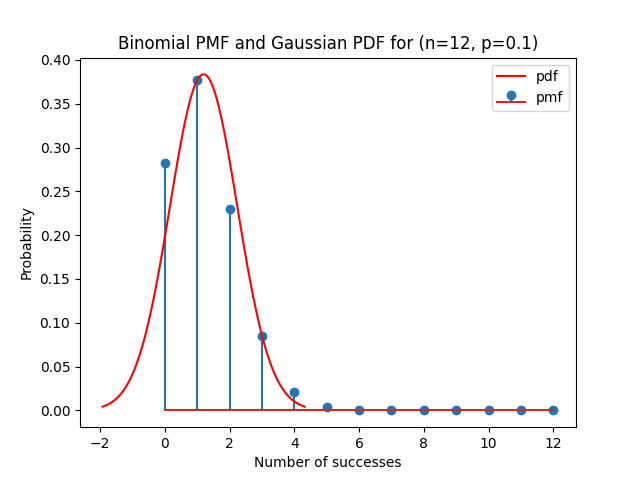
\includegraphics[width=\columnwidth]{./figs/graph.png}
\end{figure}
\\
\\\textbf{Comparision of Answers obtained from Binomial Distribution and Gaussian Distribution}
\\Binomial Distribution converges to Gaussian Distribution when the size of sample space is large.
\\If the following condition is satisfied then the Binomial distribution converges to Gaussian Distribution
 \begin{align}
    np\brak{1-p}\geqslant 10
    \end{align}
From Given
 \begin{align}
    n&=12\nonumber\\
    p&=0.1\nonumber
    \end{align}
Therefore LHS of the above condition becomes
 \begin{align}
    np\brak{1-p}&=12\times0.1\times0.9=1.08\nonumber\\
    1.08 &< 10\nonumber
    \end{align}
Therefore the above condition is not satisfied and there would be significant difference in the probabilities calculated by using Binomial Distribution approach and Gaussian Distribution approach.(here, as the size of sample space is low the Binomial approach gives more accurate answer and the probability from Gaussian Distribution approach is significantly lower than the actual probability)
\\Let 'N' be the size of sample space for the Binomial Distribution to converge to Gaussian Distribution, then
\begin{align}
    N\brak{0.1}\brak{0.9}&\geqslant 10\nonumber\\
    N&\geqslant \frac{10}{0.09}\nonumber\\
    N&\geqslant 111.11
    \end{align}
Therefore the size of Sample Space should be atleast $112$.
\end {document}